\documentclass[12pt]{article}
\usepackage[a4paper, left = 1cm, right = 1cm, top = 1cm, bottom = 1cm]{geometry}
\usepackage{dsfont}
\usepackage[fleqn]{amsmath}
\usepackage{amssymb,amstext}
\usepackage{graphicx}
\begin{document}
%\setcounter{secnumdepth}{0}
\thispagestyle{empty}

$$
\lim
$$


\begin{center}
	Universidade Federal da Paraíba \\
	Departamento de Estatística \\
	Probabilidade IV \\
	Atividade 1 - teoria de conjuntos (1 ponto) \\
	Paulo Ricardo S. Campana \\
\end{center}

\section{} \[
	B = \left\{ x \; ; \; x > \frac{9}{4} \text{ e } x < \frac{6}{5} \right\} \text{ e }
\] \[
	D = \left\{ x \; ; \; x \text{ é divisível por } 0 \right\}
\]

\section{} \[
	\begin{array}{l}
		\mathcal{P}(A) = \big\{ \\
		\hspace{+16pt} \varnothing \\
		\hspace{+16pt} \{a\}, \{b\}, \{c\}, \{d\}, \\
		\hspace{+16pt} \{a,b\}, \{a,c\}, \{a,d\}, \{b,c\}, \{b,d\}, \{c,d\}, \\
		\hspace{+16pt} \{a,b,c\}, \{a,b,d\}, \{a,c,d\}, \{b,c,d\} \\
		\hspace{+16pt} \{a,b,c,d\} \\
		\big\} \\
	\end{array}
\]

\section{}
	\begin{tabular}{rrl}
		\quad\qquad & a) & V \\
		\quad\qquad & b) & F, \{a\} não pertence a \{a,b\}, ele é subconjunto \\
		\quad\qquad & c) & F, \{0\} possui apenas um elemento e não é $\varnothing$ \\
		\quad\qquad & d) & F, $\varnothing$ é um conjunto que não possui elementos \\
		\quad\qquad & e) & F, apenas $\varnothing$ é subconjunto de $\varnothing$ \\
		\quad\qquad & f) & V \\
		\quad\qquad & g) & V \\
		\quad\qquad & h) & V \\
		\quad\qquad & i) & V \\
		\quad\qquad & j) & F, \{\{a,b,c,d\}\} possui apenas um elemento: \{a,b,c,d\} $\neq$ \{a,b\} \\
	\end{tabular}

\section{}
	\begin{align*}
		A \cap B        &= \{b,c,d\} \\
		A \cap C        &= \{c\} \\
		B \cap C        &= \{c,e\} \\
		A \cap B \cap C &= \{c\} \\
		A \cup B        &= \{a,b,c,d,e\} \\
		A \cup C        &= \{a,b,c,d,e,f\} \\
		B \cup C        &= \{b,c,d,e,f\} \\
		A \cup B \cup C &= \{a,b,c,d,e,f\} \\
	\end{align*}
	Nenhum par de conjuntos são disjuntos pois nenhuma interseção resultou em vazio

\section{}
	\begin{tabular}{rrr}
		\hspace{+32pt} a) V \hspace{+32pt} & f) V \hspace{+32pt} & k) V \\
		\hspace{+32pt} b) F \hspace{+32pt} & g) V \hspace{+32pt} & l) V \\
		\hspace{+32pt} c) F \hspace{+32pt} & h) F \hspace{+32pt} & m) V \\
		\hspace{+32pt} d) V \hspace{+32pt} & i) F \hspace{+32pt} & n) V \\
		\hspace{+32pt} e) V \hspace{+32pt} & j) V \hspace{+32pt} & o) V \\
	\end{tabular}


\section{}
	\begin{figure}[h!]
		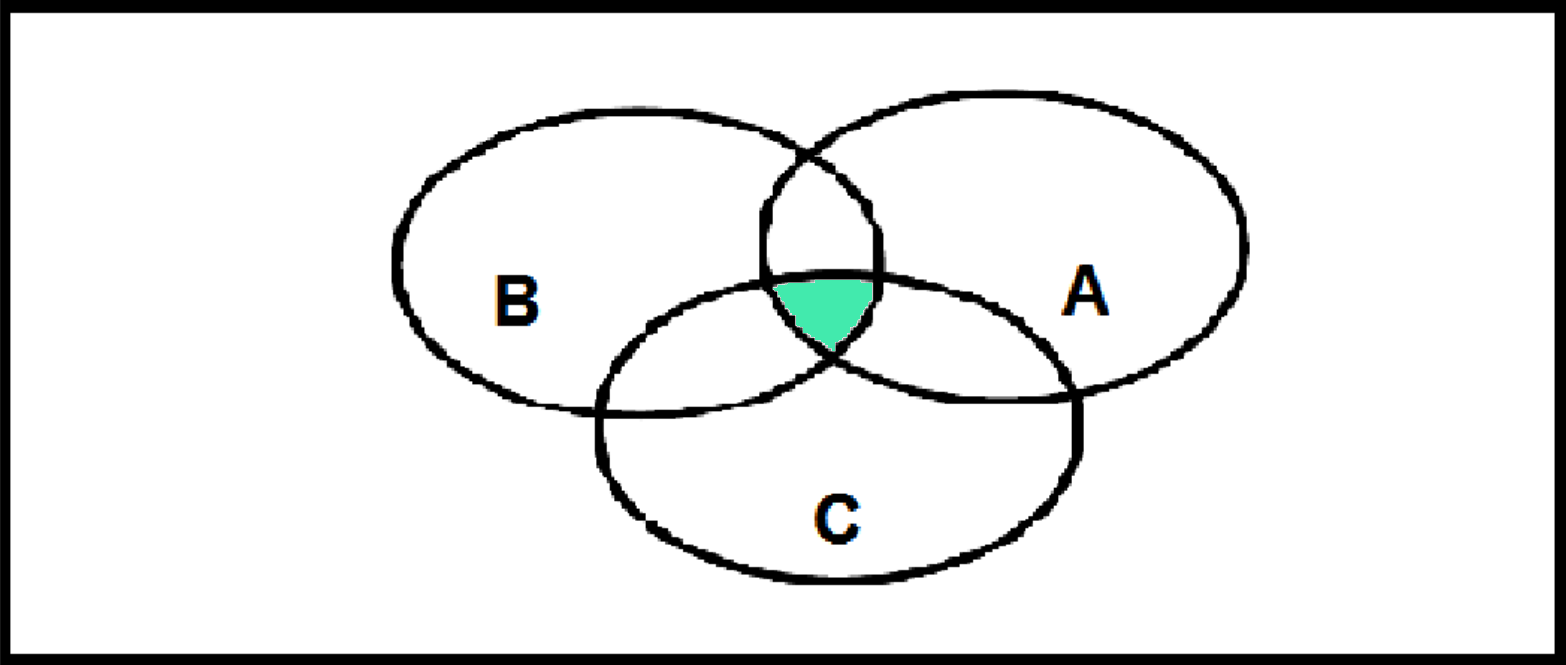
\includegraphics[scale=0.5]{q6a} $ A \cap B \cap C $ \\
		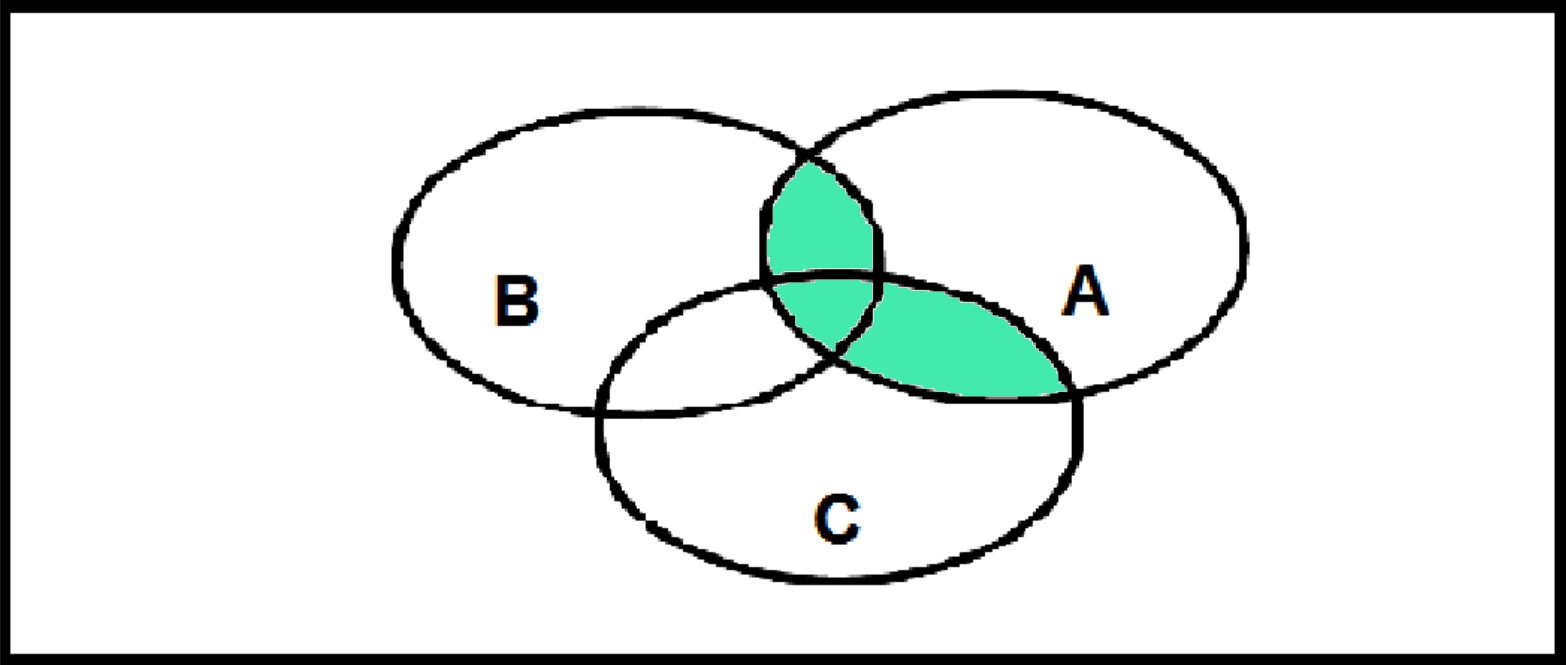
\includegraphics[scale=0.5]{q6b} $ A \cap (B \cup C) $ \\
		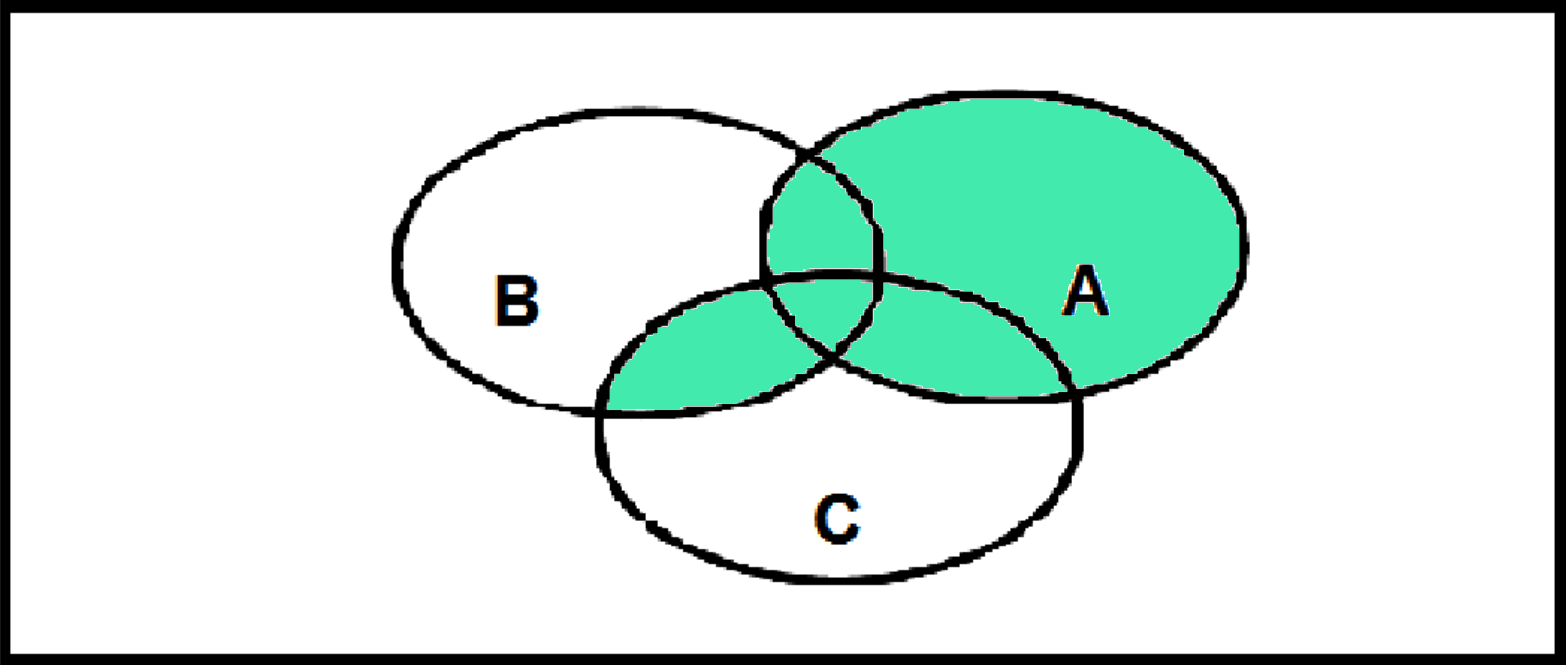
\includegraphics[scale=0.5]{q6c} $ A \cup (B \cap C) $ \\
		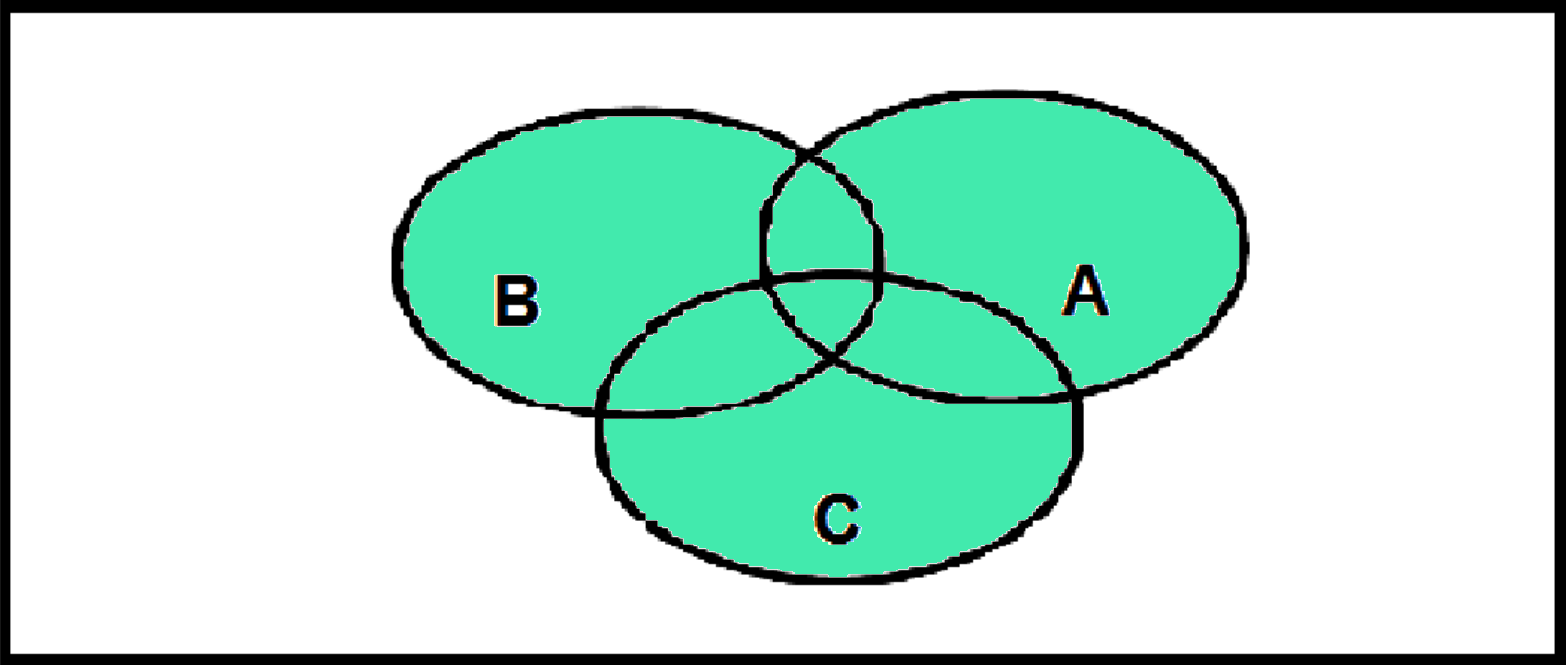
\includegraphics[scale=0.5]{q6d} $ A \cup (B \cup C) $ \\
	\end{figure}

\section{}
	\begin{align*}
		A - B &= \{a,b\} \\
		B - A &= \{e,f,g\} \\
		C - B &= \{b\} \\
		(A \cup C) - B &= \{a,b\} \\
		A - (B \cap C) &= \{a,b,c\} \\
		(A \cup B) - (A \cap C) &= \{a,c,e,f,g\}
	\end{align*}

\section{}
	\begin{figure}[h!]
		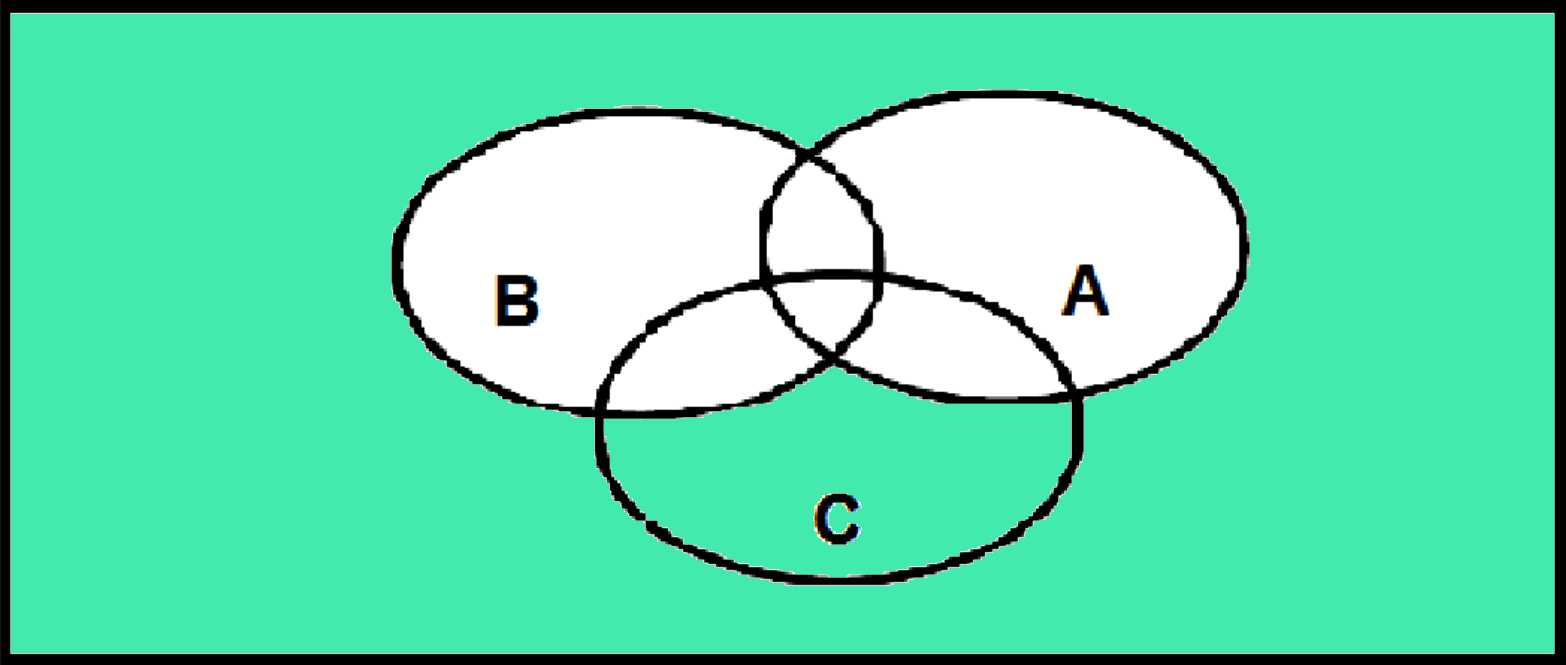
\includegraphics[scale=0.5]{q8a} $ A^c - B $ \\
		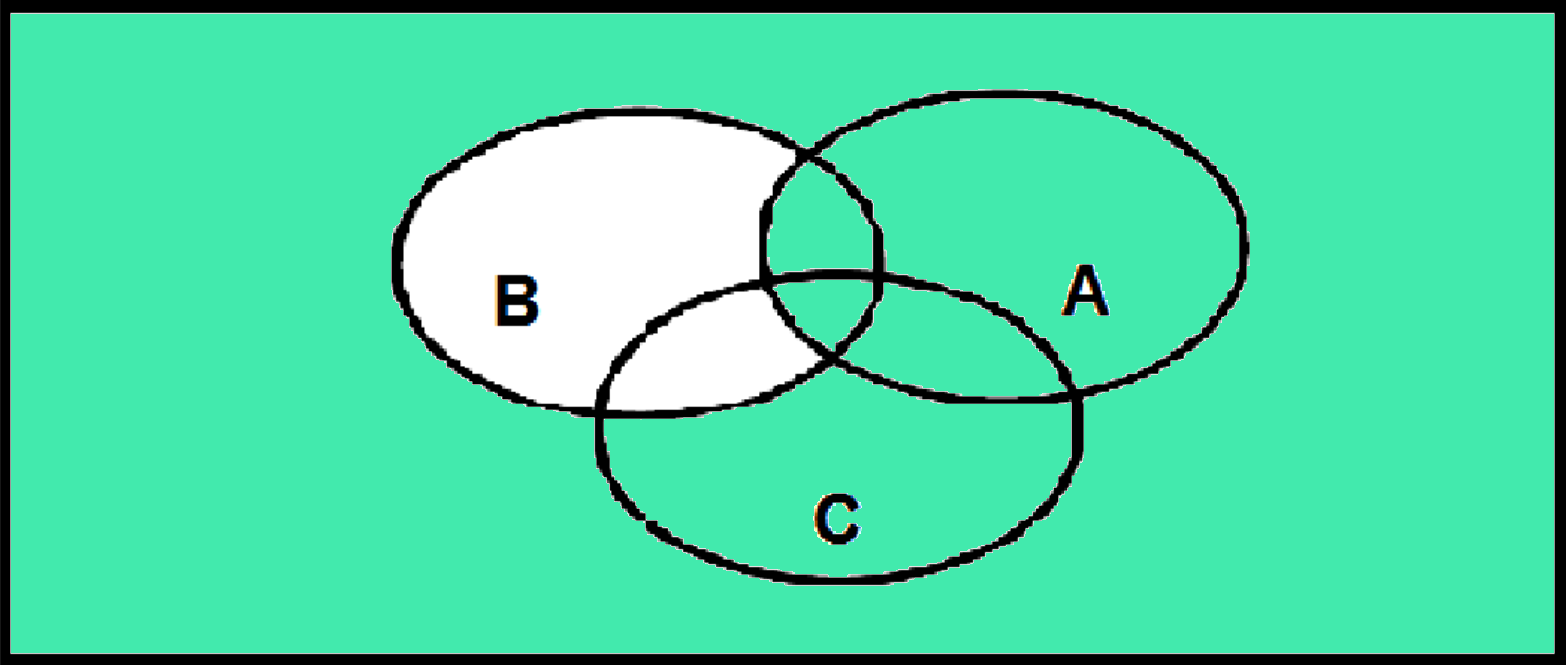
\includegraphics[scale=0.5]{q8b} $ B^c \cup A $ \\
		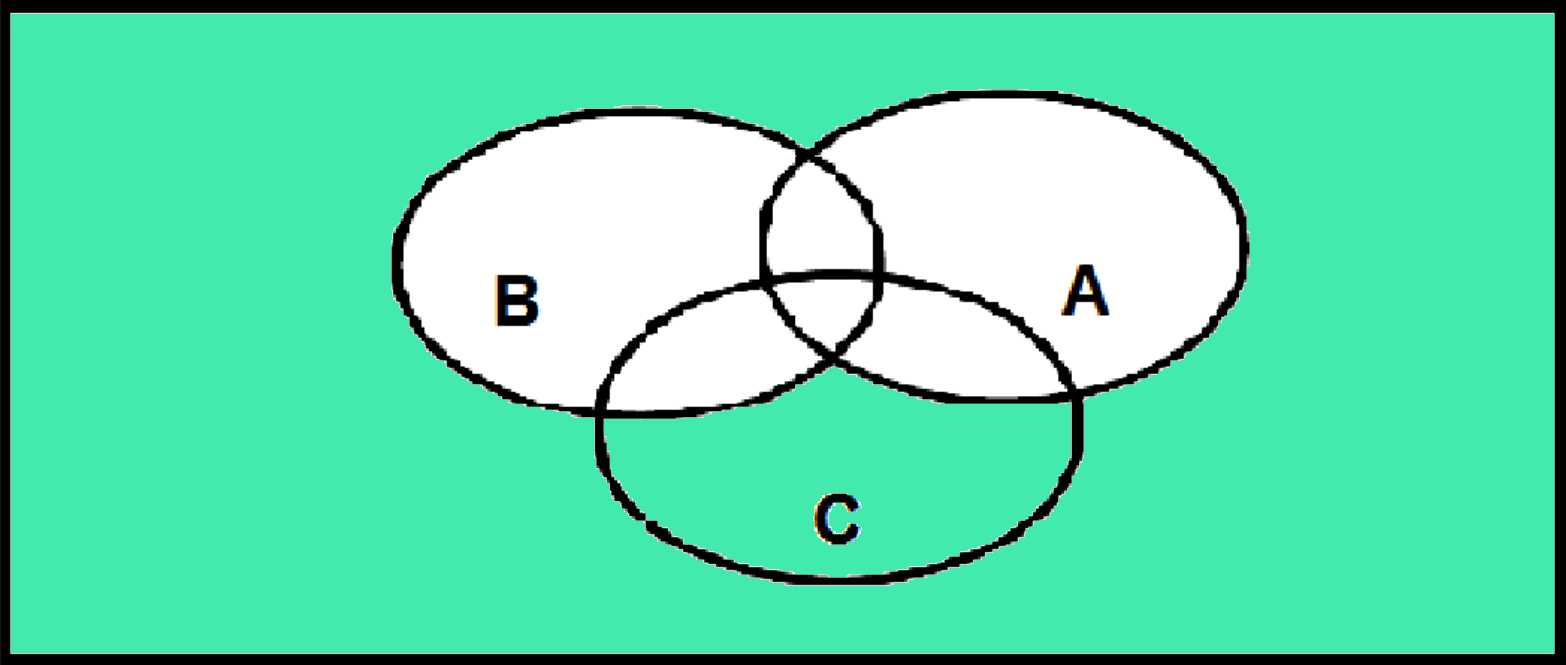
\includegraphics[scale=0.5]{q8c} $ (A \cup B)^c $ \\
		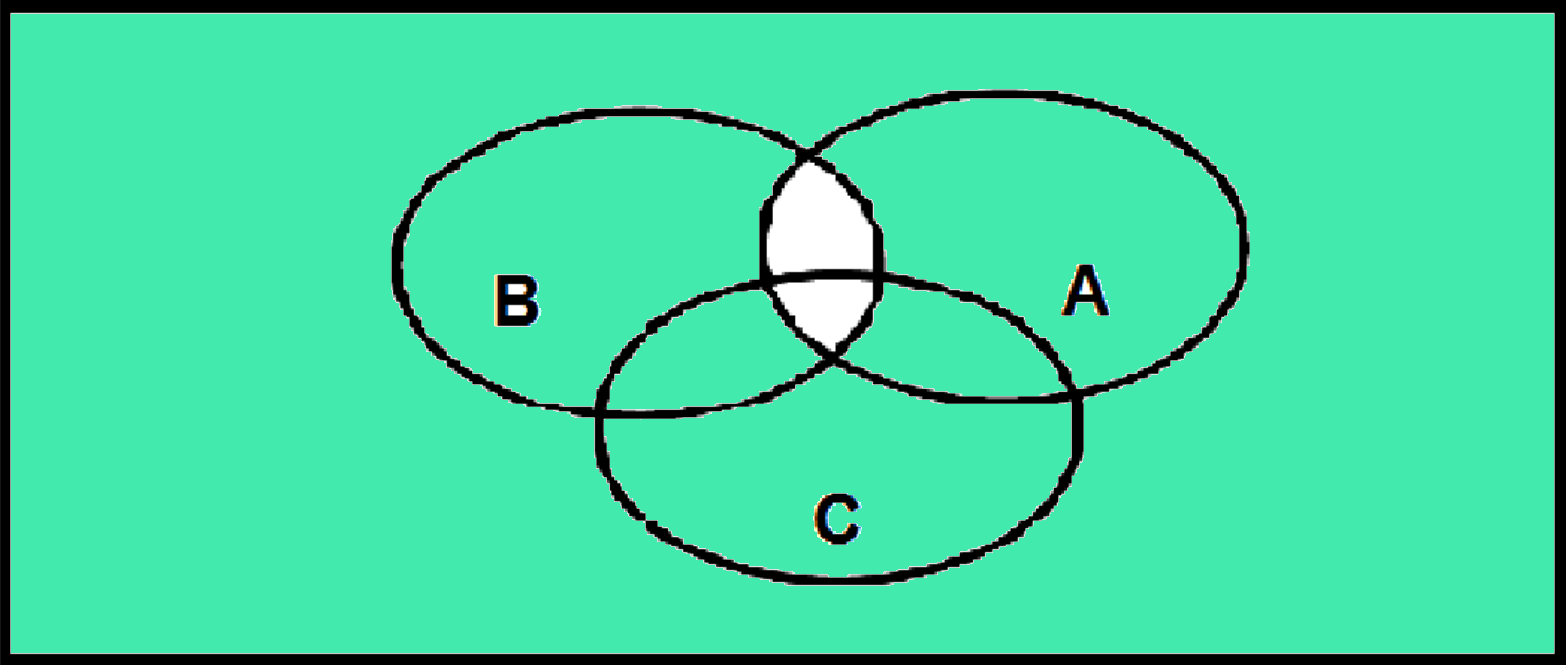
\includegraphics[scale=0.5]{q8d} $ (A \cap B)^c $ \\
		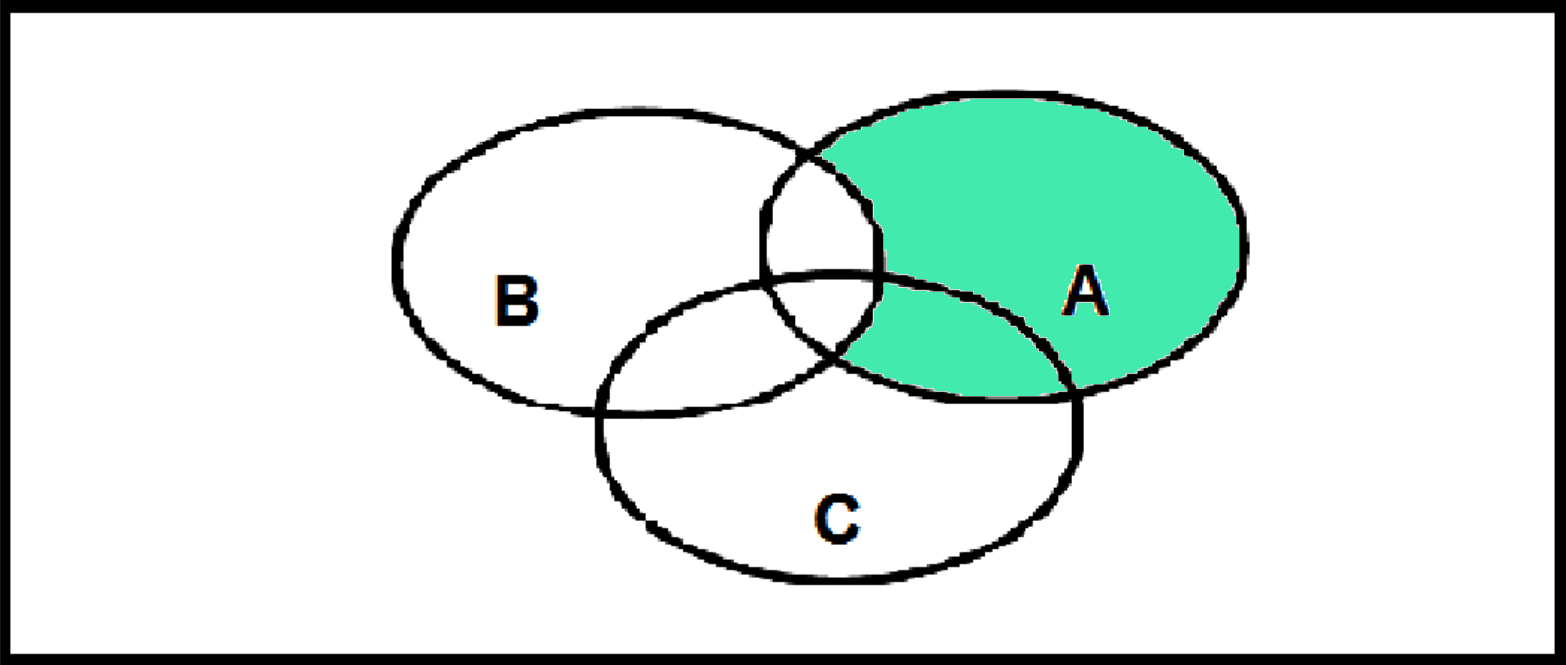
\includegraphics[scale=0.5]{q8e} $ B^c \cap A $ \\
		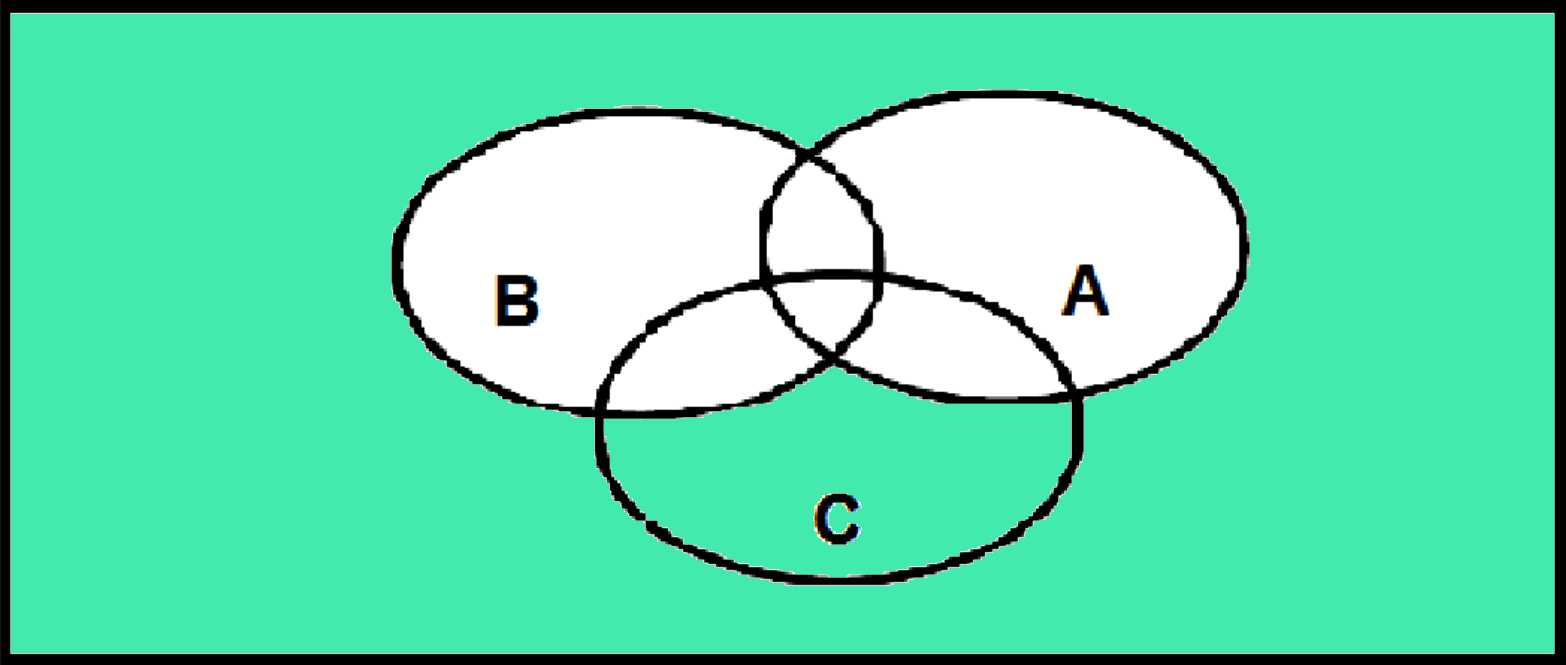
\includegraphics[scale=0.5]{q8f} $ A^c - (A \cup B) $ \\
	\end{figure}

\newpage

\section{} \[
	\text{a) } (A - C) \cup (B - C) =
	(A \cap C^c) \cup (B \cap C^c) =
	(A \cup B) \cap C^c =
	(A \cup B) - C
\] \[
	\text{b) } (A - C) \cap (B - C) =
	(A \cap C^c) \cap (B \cap C^c) =
	(A \cap B) \cap C^c =
	(A \cap B) - C
	\hfill \blacksquare
\]

\section{} \[
	A \cap (B - A) =
	A \cap (B \cap A^c) =
	(A \cap A^c) \cap B =
	\varnothing \cap B =
	\varnothing
	\hfill \text{são disjuntos}
\] \[
	A \cup (B - A) =
	A \cup (B \cap A^c) =
	(A \cup B) \cap (A \cup A^C) =
	(A \cup B) \cap U =
	A \cup B
	\hfill \blacksquare
\]

\section{}
	\begin{align*}
		A \cup B &= [0,5] \\
		A \cap B &= (3,5) \\
		B \cup C &= (2,5] \\
		C \cup (A \cap B) &= (2,5) \\
	\end{align*}


\end{document}